\begin{figure}
 \begin{subfigure}[b]{0.5\textwidth}
        \centering
        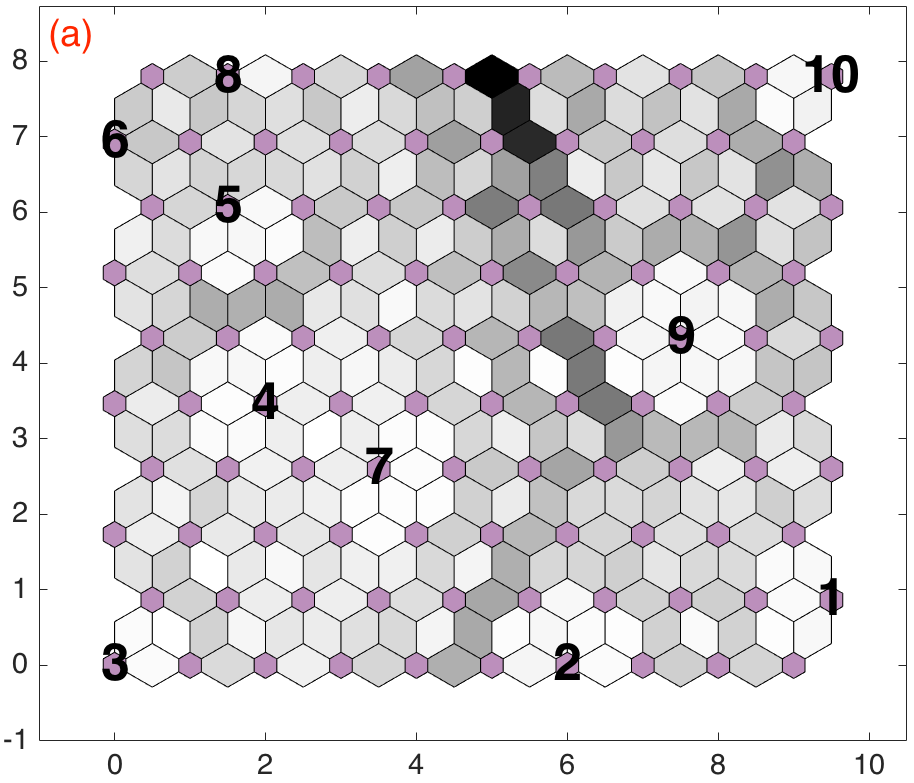
\includegraphics[width=\textwidth]{../../images0.01/M31/2D/image_subsets/subset9_dist_with_hits_t.png}
    \end{subfigure}
    \hfill
    \begin{subfigure}[b]{0.5\textwidth}
    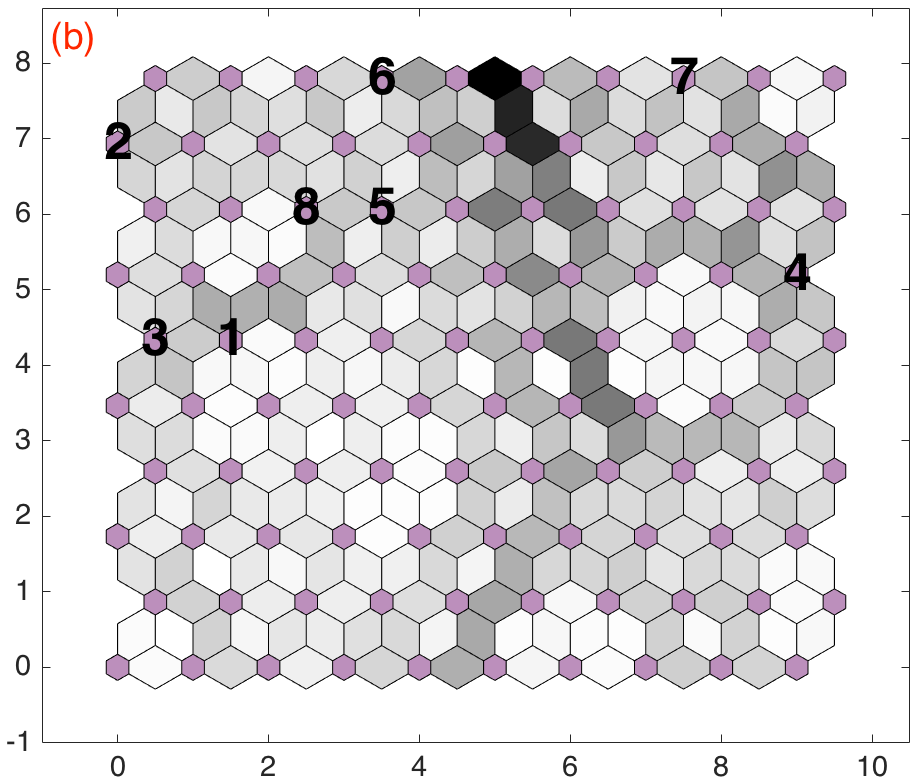
\includegraphics[width=\textwidth]{../../images0.01/M31/2D/image_subsets/subset9_dist_with_hits_v.png}
    \end{subfigure}
    \caption{Similar to Fig.~\ref{fig: all_derived_ones}, here we show up: the result from subset of data in M31 which is similar to data in M101; Down: the same network of up, but the input data are from M101.}
    \label{fig: subset9}
\end{figure}
